\section{Question 1}

\begin{verbatim}
Analyze the space and time complexity of your approach to dynamic
tracing & subsequent type inference for Typed Clojure.  Are you able
to bound space use at all by reducing traces as they are collected?
Please analyze a related system, Daikon
(https://plse.cs.washington.edu/daikon/), along the same lines.  How
expressive are Daikons invariants compared to yours?  How much space
and runtime overhead does it impose?  If Daikon's inferred invariants
were to become part of a (refinement) type system, how powerful would
it need to be?
\end{verbatim}

\pagebreak

\subsection{Dynamic tracing Performance}

To avoid the full cost of naive dynamic tracing, we leverage several
known techniques from the higher-order contract checking literature.

\subsubsection{Space complexity of dynamic tracing}

The space complexity of dynamic tracing in Typed Clojure is similar
to proxy-based higher-order contract checking.

Map and function wrappers are space-efficient with respect to the stack, with
redundant wrapper of the same type collapsing to at most one level of wrapping.

Some structural sharing of tracking data helps reduce the memory footprint
of the tracking results. Specifically, the original source of a value
is stored in a ``path'' (similar to a blame label in contract systems),
and appending to this path uses constant heap space since it is represented
using a immutable vector with structural sharing.

%The heap size of the tracking data is linear in the number of observed
%tracking points.

%\subsubsection{Benchmarks}
%
%We use several small benchmarks to demonstrate the space-efficiency of
%function wrappers, and the linear nature of the tracking data.

\subsubsection{Time complexity of dynamic tracing}

Most tracked Clojure collections are traversed lazily as they are used,
so incurs a $O(1)$ cost to each lookup.
This includes (potentially infinite) lazy sequences and hash maps.
Vectors are not currently lazily traversed, and we have not tried any vector-heavy
benchmarks to observe the performance effect (but we hypothesize matrix-heavy
code would suffer from a significant tracking penalty).

Functions are similarly wrapped a la higher-order contract checking and tracked when invoked,
so incur an overhead on every invocation.
Non-Clojure Objects simply record their class (including arrays).

\pagebreak

\subsection{Space complexity of type inference}

The type inference algorithm uses a linear amount of memory with respect
to the number of distinct HMap types in the input.
At its largest space usage, the algorithm creates a new alias for each HMap object.

However, aliases consist of a symbol and an entry in a hash-map, so the constant
factors are small.

The algorithm also can use more space as more samples are processed. For example,
a large union type could be accumulated by combining several samples.

\subsection{Time complexity of type inference}

\begin{figure}
\begin{mdframed}
\begin{description}
  \item [I] number of collected inference results
  \item [U] maximum number of union members (unordered types)
  \item [D] maximum depth of types
  \item [W] maximum width of non-union types (ordered types) (eg. HMap entries, function positions)
  \item [A] number of aliases in alias environment (reachable from the type environment)
\end{description}
\end{mdframed}
\caption{Reference for variables used in time complexity analysis}
\label{time-complexity-vars}
\end{figure}

To analyze the time complexity of dynamic type inference (after
gathering samples), we reference several variables 
defined in Figure~\ref{time-complexity-vars}.
The variable \texttt{I} denotes the number of samples
collected during dynamic tracing. The variable \texttt{U}
denotes the maximum width of a union during the entire execution
of type inference.
The maximum depth and width of non-union types are denoted by
\texttt{D} and \texttt{W} respectively.
Finally, \texttt{A} references the number of (reachable) aliases in the
alias environment.

The entire algorithm is split into several passes, many of which
rely on the \texttt{join} function, which we analyze in Section~\ref{join}.

First, a naive type environment is generated. Two approaches
are analyzed, 
one slow (Section~\ref{naive-gamma-slow}),
and one fast (Section~\ref{naive-gamma-fast}).
The implementation uses the second version in practice.

Then several passes are applied to the resulting type and
alias environments. First $squash\_vertically$
(Section~\ref{squash-vertically}) creates local recursive
types.
Then $squash\_horizontally$ (Section~\label{squash-horizontally})
merges similar recursive types that occur in different type/alias
environment entries.
The overall time complexity is summarized in Section~\ref{overall-time-complexity}.

\subsubsection{Join}
\label{join}
\begin{verbatim}
join(D, W, U) = O(D * max(W, U^2))
\end{verbatim}

Joining two union types involves joining all the combinations of the union members ($U^2$ joins).

Joining two non-union types that are not the same sort of type is constant.

Joining two non-union types that are the same sort of type joins
each of the members of its types pairwise, of which the maximum number is $W$.

A maximum number of $D$ recursive joins can occur, and $max(W, U^2)$ work is done
at each level, so time complexity is $O(D * max(W, U^2))$.

\subsubsection{Naive type environment creation}
\label{naive-gamma-slow}

1. Build naive type environment.
   Folds over inference results, `update' from the top of each type.
   Naive algorithm traverses depth/width of type 

\begin{verbatim}
naive(I, D, W, U) = O(I * (D + join(D, W, U)))
\end{verbatim}

Iterate over each inference result, there are $I$ of them.

Build up a sparse type from the inference result, maximum depth $D$.

Join this type with the existing type taking $join(D, W, U)$.

Since we do $(D + join(D, W, U))$ work for each result, time complexity
is $O(I * (D + join(D, W, U)))$.

\subsubsection{Naive type environment creation (optimized)}
\label{naive-gamma-fast}

1. Build naive type environment (optimized)
  Group inference results by path prefixes. Then join the groups
  from the longest prefixes first, and use previous results to avoid
  recalulating joins.

\[
optimized\Gamma(I, D, W, U) = O(I * (D + join(D, W, U)))
\]

\subsubsection{Squash Vertically}
\label{squash-vertically}
Iterate down each type in the type environment and merge similarly "tagged"
maps, resulting in a possibly recursive type.

Each iteration involves:

\begin{itemize}
  \item \emph{alias-hmap-type} Ensure each HMap in the current type corresponds to an alias.
		\begin{itemize}
			\item Involves walking the current type once
			\item $alias\_hmap\_type(D,W,U) = O(D*W*U)$
		\end{itemize}
  \item \emph{squash-all} Each alias mentioned in the current type is "squashed".
		\begin{itemize}
			\item At worst, could join each alias together.
			\item $squash\_all(A,D,W,U) = O(A*join(D, W, U))$
		\end{itemize}
\end{itemize}

\[
squash\_vertically(\Gamma, A, D, W, U) = O(|\Gamma| * (D*W*U + A*join(D, W, U)))
\]

\subsubsection{Squash Horizontally}
\label{squash-horizontally}

Iterate over the reachable aliases (from the type environment)
several times, merging based on several criteria.

These are the passes:

\begin{itemize}
	\item \emph{group-req-keys} Merge HMap aliases with similar keysets, but
		don't move tagged maps
		\begin{itemize}
			\item First groups aliases into groups indexed by their keysets, then
					joins those groups together, merging each group into its own alias.
			\item $group\_req\_keys(A,D,W,U) = O(A + A*join(D*W*U))$
		\end{itemize}
	\item \emph{group-likely-tag} Merge HMap aliases with the same tag key/value pair
		\begin{itemize}
			\item First groups aliases into groups indexed by their likely tag key/value, then
					joins those groups together, merging each group into its own alias.
			\item $group\_likely\_tag(A,D,W,U) = O(A + A*join(D*W*U))$
		\end{itemize}
	\item \emph{group-likely-tag-key} Merge HMap aliases with the same tag key.
			  This gathers HMaps with the same tag key into the large unions seen in the algorithm's
				final output.
		\begin{itemize}
			\item First groups aliases into groups indexed by their likely tag key, then
					joins those groups together, merging each group into its own alias.
			\item $group\_likely\_tag\_key(A,D,W,U) = O(A + A*join(D*W*U))$
		\end{itemize}
\end{itemize}

\begin{align*}
squash\_horizontally(\Gamma, A, D, W, U) = O(&group\_req\_keys(A,D,W,U)\\
								  													 &+ group\_likely\_tag(A,D,W,U) \\
								  												   &+ group\_likely\_tag\_key(A,D,W,U))
\end{align*}

\subsubsection{Overall time complexity}
\label{overall-time-complexity}
The overall time complexity is the sum of the previous passes.

\begin{align*}
alg(\Gamma,A,I,D,W,U) = O(&optimized\Gamma(I, D, W, U) \\
												  &+ squash\_vertically(\Gamma, A, D, W, U)\\
													&+ squash\_horizontally(\Gamma, A, D, W, U))
\end{align*}

Based on this analysis, we have a few observations:

\begin{itemize}
\item the larger the number of aliases, the slower the algorithm
	\begin{itemize}
		\item both the phases that merge aliases traverse and potentially
					the aliases in the type environment together.
	\end{itemize}
\item the larger the size of unions, the slower the algorithm
	\begin{itemize}
		\item \emph{join} is quadratic in the size of the largest union.
	\end{itemize}
\end{itemize}

\subsection{Benchmarks}

To test the time complexity of the implementation of the type reconstruction
algorithm, we devise several benchmarks.

The benchmarks are designed to emperically determine the influence of the
size of the largest union type on the time complexity of the type reconstruction
algorithm.

\subsubsection{Benchmark 1: 2 tags}

The first benchmark generates deep inputs using one of 2 "tagged" maps.
This is equivalent to seeding the algorithm with
a large Lisp-style list with cons/null constructors.

Since there is only one interesting tagged map, the early phases of the
algorithm should collapse (or "squash") these repeated tag occurrences
into a small (recursive) union, thus minimizing the size of the largest
union in the later stages of the algorithm.

Benchmark 1 takes as input the number of "cons" tagged maps to wrap
around a "null" tag. For example, input 5 starts the algorithm with
the type

\begin{verbatim}
'{:tag ':cons,
  :cdr '{:tag ':cons,
          :cdr '{:tag ':cons,
                :cdr '{:tag ':cons, 
                       :cdr '{:tag ':cons, 
                              :cdr '{:tag ':null}}}}}}
\end{verbatim}

The final output of the algorithm is a recursive type with 2 tags.

\begin{verbatim}
(defalias Tag (U '{:tag ':cons, :cdr Tag} '{:tag ':null}))
\end{verbatim}

All inputs to Benchmark 1 greater than 0 result in this same calculated type.

\subsubsection{Benchmark 2: Many tags}

The second benchmark forces the largest union to be linear to the depth
of the input type. It achieves this with a similar approach to Benchmark 1,
except every level of the initial type is tagged with a unique type.

Since the recursive type reconstruction only collapses identically-tagged
maps, we preserve a large union throughout the algorith.

We demonstrate the behavior of Benchmark 2 at depth 5. This is the initial
type we use to recover types from:

\begin{verbatim}
'{:tag ':cons5,
  :cdr '{:tag ':cons4,
         :cdr '{:tag ':cons3,
                :cdr '{:tag ':cons2, 
                       :cdr '{:tag ':cons1,
                              :cdr '{:tag ':null}}}}}}
\end{verbatim}

And, since the input has 6 unique tags, our final recursive type has a
recursive union of width 6.

\begin{verbatim}
(defalias
  Tag
  (U
    '{:tag ':cons1, :cdr Tag}
    '{:tag ':cons2, :cdr Tag}
    '{:tag ':cons3, :cdr Tag}
    '{:tag ':cons4, :cdr Tag}
    '{:tag ':cons5, :cdr Tag}
    '{:tag ':null}))
\end{verbatim}

The width of the reconstructed type is linear in the depth of the input type.
For example, Benchmark 2 with depth 10 results in:

\begin{verbatim}
(defalias
  Tag
  (U
    '{:tag ':cons1, :cdr Tag}
    '{:tag ':cons2, :cdr Tag}
    '{:tag ':cons3, :cdr Tag}
    '{:tag ':cons4, :cdr Tag}
    '{:tag ':cons5, :cdr Tag}
    '{:tag ':cons6, :cdr Tag}
    '{:tag ':cons7, :cdr Tag}
    '{:tag ':cons8, :cdr Tag}
    '{:tag ':cons9, :cdr Tag}
    '{:tag ':cons10, :cdr Tag}
    '{:tag ':null}))
\end{verbatim}

\subsubsection{Results}

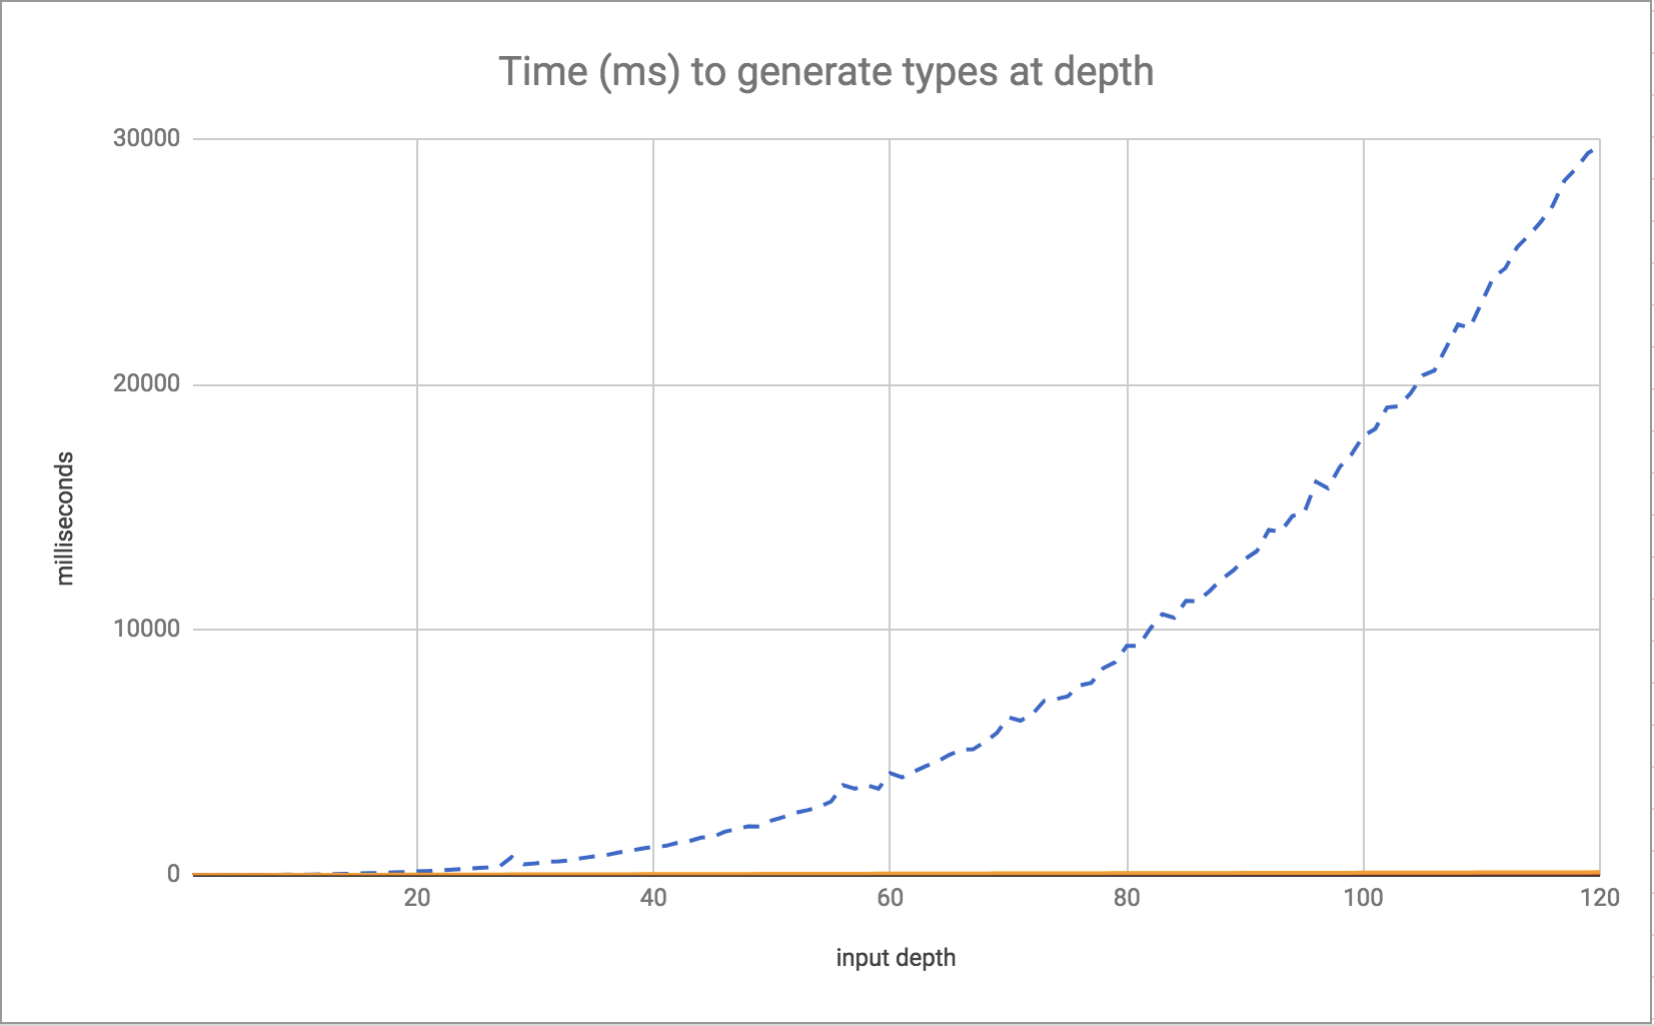
\includegraphics[width=\textwidth]{tagged-untagged-depth-bench120}

Benchmark 1 is represented by the red solid line, benchmark 2 by the
blue dotted line.

The graph shows the performance of Benchmark 1 is constant, because
the width of the largest union is always 2\ in an early phase of the reconstruction
algorithm.

The results for Benchmark 2 show the reconstruction algorithm is quadratic
with respect to the size of the largest union.

These observations are consistent with the prior theoretical analysis.

\subsection{Can space use be bounded by reducing traces as collected?}

Traces in Typed Clojure's dynamic analysis are accumulated online, and then
folded into a type environment offline. However, this fold operation is commutative
with respect to the order of traces, so performing this fold online would
eliminate the need to store traces in memory.

Space is reduced further, then, by leveraging \texttt{join} to eagerly simplify
the accumulated type environment. For example, heterogeneous maps with similar
keysets could merged, possibily using optional key entries, saving space by
preventing very large redundant unions.

It is unclear if it is possible to perform more sophisticated analyses online,
in particular the recursive type reconstruction algorithm. Since the resulting
annotations are very compressed compared to intermediate points in the analysis,
fully or partially performing this analysis online may drastically decrease space
usage where recursively defined maps are used, and very deep examples are found.

\subsection{Daikon}

Daikon is a related system to Typed Clojure's dynamic type inference.
However, Daikon is built for ``invariant detection'', while our system
is designed for ``dynamic type inference'' or ``value profiling''.

There are two common implementation strategies for such tools. The first
strategy, ``ruling-out'' (for invariant detection), assumes all invariants are true 
and then use runtime analysis results to rule out
impossible invariants. The second ``building-up'' strategy (for dynamic type inference)
assumes nothing and then uses runtime analysis results to build up invariant/type knowledge.

Both strategies have different space behavior with respect to representing
the set of known invariants.
The ruling-out strategy typically uses a lot of memory at the beginning,
but then can free memory as it rules out invariants. For example, if
\texttt{odd(x)} and \texttt{even(x)} are assumed, observing \texttt{x = 1}
means we can delete and free the memory recording \texttt{even(x)}.
Alternatively, the building-up strategy uses the least memory storing
known invariants/types at the beginning, but increases memory usage
as more the more samples are collected. For example, if we known
\texttt{x : Any}, and we observe \texttt{x = "a"} and \texttt{x = 1}
at different points in the program, we must use more memory to
store the union \texttt{x : String $\cup$ Integer} in our set of known invariants.

Examples of invariant detection tools include Daikon \cite{Ernst06thedaikon},
DIDUCE \cite{hangal2002tracking}, and Carrot \cite{pytlik2003automated}, and
typically enhance statically typed languages with more expressive types or contracts.
Examples of dynamic type inference include Rubydust \cite{An10dynamicinference},
JSTrace \cite{saftoiu2010jstrace}, and TypeDevil \cite{pradel2015typedevil},
and typically target untyped languages.

There is some overlap between invariant detection and dynamic type inference
tools. Usually, invariant detection detects very expressive relationships
between program variables; for example, for array \texttt{a} and index
\texttt{i} variables, a derived invariant might be \texttt{0 < a[i]}.
On the other hand, dynamic type inference (or value profiling) often just records
basic nominal or structural type information---it is generally applied to untyped
languages where basic static type information is absent.

\subsubsection{Daikon's expressivity vs Typed Clojure's dynamic inference}

Daikon can reason about very expressive relationships between variables
using properties like ordering ($x < y$), linear relationships ($y = ax + b$),
and containment ($x \in y$). It also supports reasoning with ``derived variables''
like fields ($x.f$), and array accesses ($a[i]$).

Typed Clojure's dynamic inference can record heterogeneous data structures
like vectors and hash-maps, but otherwise cannot express relationships
between variables.

There are several reasons for this. The most prominent is that Daikon
primarily targets Java-like languages, so inferring simple type information
would be redundant with the explicit typing disciplines of these languages.
On the other hand, the process of moving from Clojure to Typed Clojure
mostly involves writing simple type signatures without dependencies
between variables. Typed Clojure recovers relevant dependent information
via occurrence typing, and gives the option to manually annotate necessary
dependencies in function signatures when needed.

\subsubsection{Space/time overhead of Daikon's dynamic tracing}

Performance of dynamic tracing is not directly addressed in the Daikon
literature, who only provide complexity analyses and optimizations for storing
and checking invariants \emph{after} samples have been collected.

I have manually examined Chicory (the Java front-end to Daikon) to see how
dynamic tracing is implemented.
I found that Daikon records the value of all variables in scope
at each method entry/exit point \footnote{Implemented in \texttt{daikon.chicory.DaikonVariableInfo}}.
Then, to record values in Daikon, the following algorithm is used:

\begin{itemize}
  \item If the value is a Java primitive, record its value.
  \item If the value is an array, traverse its contents and record identity hash codes
    and/or primitive values.
  \item Otherwise, record the class of the current object.
\end{itemize}

Notice this algorithm is non-recursive---while arrays are traversed eagerly, they
are only traversed one level via an identity hash code summary (the closest equivalent to
pointer addresses on the JVM).
This is significantly different to Typed Clojure's value tracing algorithm,
which recursively (but lazily) traverses potentially-deep data structures.

Another difference is that Typed Clojure's dynamic tracing only tracks
values for arguments/returns of a function, and ignores any variables
that in are scope. There are several reasons behind this decision.
First, Java-like object-oriented languages use fields as implicit
arguments to methods, and Daikon distinguishes method-level, and class-level
invariants which is achieved by checking class-level invariants during
method calls.
In Clojure, methods are replaced with pure functions (their output is defined only by the
explicitly passed arguments), so the method/class-level distinction is
not applicable.

Second, Daikon chooses to reason about local mutation in Java-like languages,
and so must record the values of the same variables different program points
to observe mutation. However, local unsynchronized mutation is non-idiomatic
in Clojure so re-tracking variables is almost always redundant---mutation is
often via synchronized global variables that can be instrumented once-and-for-all.

\subsubsection{Space/time overhead of Daikon's type inference}

The overhead of likely invariant detection
is described by Perkins and Ernst~\cite{Perkins04efficientincremental}.
They analyze the overhead of storing and checking the set of
invariants that are currently true.
Their presentation includes a simple incremental algorithm that
features no optimizations, then they propose several candidate
optimizations and emperically compare the performance of each
approach.

The space complexity of the simple incremental algorithm is dominated 
by the size of the grammar of properties. For example, if the grammar
of properties consists of $=$ and $even$, with
3 variables $x$, $y$, $z$, the initial (and largest) set of invariant assumptions
is $x = y$, $y = z$, $x = z$, $even(x)$, $even(y)$, and $even(z)$.
For reference, Daikon enables 152 properties by default, with
12 ``derived variables'', the latter of which provide properties on composite variables
like $a[x] = a[z]$. After a static analysis pass ruling out nonsensical invariants,
the space usage is at least $O(v^9)$, where $v$ is the number of variables in scope.

The time complexity of \emph{checking} invariants for each sample
is similarly dominated by the size of the grammar of properties.
They note, however, most invariants are removed quickly (after
$O(1)$ samples), so performance improves as more samples
are collected.

\subsubsection{Checking Daikon's invariants in a refinement type system}

Daikon has expressive invariants, but can they be statically verified?
Yes, in fact Daikon supports generating annotations for a Java-based
theorem prover called Simplify~\cite{Detlefs03simplifya}.

Simplify implements the following theories.

1. The theory of equality, \texttt{=}

2. The theory of arithmetic with functions \texttt{+}, \texttt{*}, \texttt{-},
   and relation symbols \texttt{>}, \texttt{<}, \texttt{<=}, and \texttt{>=}.

3. The theory of maps with two functions \texttt{select} and \texttt{store} (ie. get/set),
   and two additional axoims.

4. Partial orders. % (?)

These could be encoded in Dependent Typed Racket, since it supports propositions
in linear arithmetic constraints about variables, pairs, car, and cdr.

% Notes:
%  Java implementation:
%    Chicory does instrumentation on JVM bytecode
%     instrument_all_methods: https://github.com/codespecs/daikon/blob/master/java/daikon/chicory/Instrument.java#L409
%      add_entry_instrumentation
%     - https://github.com/codespecs/daikon/blob/master/java/daikon/chicory/Instrument.java#L825
%      add_return_instrumentation
%       - instruments return statements
%      - https://github.com/codespecs/daikon/blob/master/java/daikon/chicory/Instrument.java#L675
%     daikon.chicory.Runtime
%      - contains wrappers for values that are rewritten to?
%      - Runtime.enter(...) is called at the top of every wrapped method
%      - `dtrace_writer` records inference results
%      daikon.chicory.DaikonVariableInfo
%      - actually traverses values here
%      - arrays are traversed eagerly, but only one level
%        - subsequent levels use identityHashCode summaries

